\chapter{Infografiche}
\label{cap:studio_infografiche}
\intro{In questo capitolo verranno esaminate le caratteristiche funzionali e di design delle infografiche e 
presentate le loro applicazioni. Verrà inoltre fornita una classificazione delle infografiche basata sulla 
loro struttura e output visivo.}\\

\section{Definizione e applicazioni}
\subsection{Cos'è un infografica e in cosa si distingue dalla data visualization}
%cap1: Design della mente – infografica e data viz” di Paolo Bottazini, Michele Gotuzzo 
Analogamente alla \gls{datavizg}, le infografiche si occupano di rappresentare visivamente i dati al fine di comunicarli in maniera più semplice e accessibile.
Esse trasformano i dati in idee chiare, permettendo di inquadrare facilmente un fenomeno, una situazione o un processo, coadiuvando così la presa di decisioni ponderate sul tema presentato.
Queste idee sono generate a partire dall'interpretazione, formalizzazione e contestualizzazione dei dati, che spesso sono disomogenei per formato, tipo di contenuto e origine. Tale interpretazione ha il compito di 
svelare il significato nascosto nel \emph{dataset} e selezionare le connessioni o fenomeni più interessanti per il destinatario della comunicazione.
In altre parole, l'infografica non si limita a mostrare i dati, ma li organizza e li presenta in un modo da renderne più evidente significato e importanza.

Per raggiungere questo obiettivo, le infografiche combinano elementi testuali e grafici per presentare le informazioni; usando le parole di E. Tufte ``un'infografica mostra visivamente grandezze misurate mediante 
l'uso combinato di punti, linee, un sistema di coordinate, numeri, simboli, parole, ombreggiature e colore''. Pertanto, le infografiche rigettano la tradizione di ``purezza grafica'' (i.e. rappresentazione dei dati 
basata solo su grafici, diagrammi e mappe) imposta alla \gls{datavizg} e abbracciano, invece, un insieme molto più amplio di tecniche di comunicazione visiva, come illustrazioni, immagini, etc.
% TODO: aggiungere citazione come footnote The visual display of quantitative information, Edward Tufte [2001], Introduction, p.10
Inoltre, il focus dell'infografica non è solamente l'oggetto da rappresentare, come invece accade con la \gls{datavizg}. Infatti, le infografiche
prendono in considerazione anche il destinatario della comunicazione, scegliendo e disponendo gli elementi per costruire una narrazione.
Possiamo infatti pensare all'infografica come a una forma di racconto, di lettura che non è di per sé né imparziale né completa, ma si limita a fare luce ed esporre i punti salienti individuati nel \emph{dataset}.
%intro: “L'arte funzionale – Infografica e visualizzazione delle informazioni” di Alberto Cairo
In realtà, tale caratteristica delle infografiche è proprio ciò che maggiormente le distingue dalla \gls{datavizg}. Infatti, mentre le prime sono progettate per presentare i dati raccontandoli attraverso storie specifiche, guidando il lettore con una narrazione, la seconda
è più orientata verso l'esplorazione autonoma delle informazioni da parte del fruitore, che deve analizzare e scoprire i dati per conto proprio. 
Questa differenza nel livello di analisi richiesto si ripercuote anche sul tipo di pubblico di ciascun tipo di rappresentazione. Nello specifico, le infografiche, grazie alla loro capacità di semplificare e contestualizzare i dati, sono accessibili anche a coloro
che non possiedono capacità analitiche avanzate e, pertanto, hanno un pubblico più ampio. 

%intro: “L'arte funzionale – Infografica e visualizzazione delle informazioni” di Alberto Cairo
Nonostante queste differenze, infografiche e \gls{datavizg} sono strettamente connesse e complementari. Le infografiche, pur essendo maggiormente orientate alla narrazione, 
possono includere elementi che stimolano l'esplorazione autonoma dei dati. Allo stesso modo, le \emph{visualizzazioni dei dati} possono contenere aspetti narrativi che facilitano 
l'interpretazione.


\subsection{Applicazioni e vantaggi}
Le infografiche sono strumenti versatili che vengono utilizzati in una vasta gamma di settori e contesti, in particolare al fine 
di analizzare o presentare dati. Offrono infatti vantaggi significativi che le rendono particolarmente adatte a questi scopi.

%Infographics: The New Communication Tools in Digital Age, Waralak V. Siricharoen
Per quanto riguarda l'\textbf{analisi dei dati}, le infografiche sono utili per la cosiddetta \gls{expdataanalysisg}, dove il fruitore non ha una domanda precisa a cui sta cercando risposta, bensì 
vuole semplicemente scoprire cosa emerge di interessante dal \emph{dataset}.

Per quanto riguarda invece la \textbf{presentazione dei dati}, va da sé che le infografiche siano perfette per tale scopo, in quanto riescono attraverso una narrazione a comunicare in maniera efficace 
e abbracciare in tal modo un pubblico molto amplio.

\bigskip
\noindent In generale, quale sia l'applicazione, l'uso di infografiche consente anche di:
\begin{itemize}
    \item \textbf{Facilitare la scoperta di informazioni} nascoste e \textbf{stimolare la curiosità} per una ricerca futura;
    \item \textbf{Semplificare la comprensione}, facilitando così il raggiungimento della \emph{saggezza};
    \item \textbf{Raccontare una storia} che permetta una visione d'insieme della situazione, fenomeno o processo presentato.
\end{itemize}



\section{Classificare le infografiche}
\subsection{Metodi di classificazione}\label{subsec:info_classifica}
% file criteri_scelta_infografica_v0.1.0
Una prima classificazione delle infografiche può essere fatta \textbf{in base all'output visivo}. Nello specifico, si hanno:
\begin{itemize}
    \item \textbf{Infografiche statiche}, in cui le informazioni sono rappresentate e visibili tutte in un'unica volta, avendo così un impatto più
    veloce e immediato sul pubblico.
    \begin{itemize}
        \item Esempio: infografiche presenti nei giornali.
    \end{itemize}
    \item \textbf{Infografiche animate}, in cui le informazioni sono presentate sequenzialmente in maniera consistente oppure contengono altri tipi di animazione.
    \begin{itemize}
        \item Esempio: infografiche realizzate tramite presentazioni multimediali.
    \end{itemize}
    \item \textbf{Infografiche interattive}, in cui le informazioni sono presentate in base a scelte operate dall'utente.
    \begin{itemize}
        \item Esempio: infografiche online in cui è l'utente a selezionare il dettaglio a partire da un insieme complesso di informazioni visualizzate.
    \end{itemize}
\end{itemize}

\bigskip
\noindent Un'altra classificazione può essere fatta \textbf{in base all'obiettivo}. Nello specifico, si hanno:
\begin{itemize}
    \item \textbf{Infografiche basate su processi ordinati}, le quali vengono usate per mostrare passo dopo passo un processo o una 
    sequenza ordinata di informazioni ad esempio per insegnare qualcosa di nuovo all'utente (e.g. ricette).
    \item \textbf{Infografiche a mo' di lista}, in questo caso le informazioni sono rappresentate sotto forma di elenco testuale, eventualmente accompagnato da icone.
    Per costruzione, queste infografiche permettono di mostrare molte informazioni e, allo stesso tempo, di farle comprenderle velocemente.
    \item \textbf{Infografiche basate sul tempo}, in cui viene mostrata una sequenza cronologica di eventi, in altre parole come si evolve una storia o un soggetto nel tempo.
    Quest'ultimo è solitamente rappresentato tramite una linea, chiamata appunto ``linea del tempo''.
    \item \textbf{Infografiche basate sul confronto}, esse comparano due diversi argomenti in contrasto ponendoli uno a fianco all'altro.  Ciò ritorna molto utile per mostrare
    quali elementi i due hanno in comune oppure per quanto divergono o sono superiori/inferiori uno rispetto all'altro.
    \item \textbf{Infografiche basate su una gerarchia}, le quali vengono utilizzate per mostrare informazioni organizzate per livelli e il collegamento tra questi.
    \item \textbf{Infografiche basate su informazioni correlate poste allo stesso livello}, in cui si vuole comunicare un nuovo concetto o dare una panoramica su un argomento; infatti,
    tali infografiche sono anche dette ``Infografiche informative''. Solitamente, lo spazio viene diviso in sezioni con un proprio titolo descrittivo.
\end{itemize}


\subsection{Infographic-helper}
Come accennato in precedenza, l'infografica è una forma di racconto e, pertanto, la scelta e scrittura della storia da comunicare sono centrali nella sua costruzione.
Nel corso dello stage si è dunque voluto sviluppare uno strumento prototipale, \emph{Infographic-helper}, che potesse aiutare il ``narratore'' in tale compito.
Nello specifico, questo strumento consente di validare tale narrativa, oltre a individuarne le parti e l'obiettivo principale.

Lo strumento è disponibile a \href{http://www.overleaf.com}{questo link}.

\subsubsection{Validazione della narrativa}
Uno degli obiettivi di \emph{Infographic-helper} è garantire che la narrativa dell'infografica sia persuasiva e venga recepita efficacemente dal pubblico. 
Questi obiettivi coincidono con quelli della retorica, la quale fornisce i principi per costruire messaggi convincenti e chiari, che espongono il punto di vista del comunicatore in maniera comprensibile. 
Questi principi non solo sono applicabili alla pura comunicazione verbale, ma si rivelano utili anche per le infografiche. 
Infatti, nonostante queste siano rappresentazioni visive, esse sono comunque una forma di narrazione e comunicazione e pertanto oggetto di retorica. 

Aristotele, pioniere di quest'arte, definisce suddetti principi come \emph{ethos}, \emph{pathos} e \emph{logos}. Nello specifico:
\begin{itemize}
    \item \textbf{\emph{Ethos}}, comprende tutto ciò che stabilisce o aumenta la credibilità e autorità del comunicatore e delle fonti;
    \item \textbf{\emph{Pathos}}, comprende tutto ciò che suscita emozioni nel pubblico, che crea una connessione emotiva con gli spettatori;
    \item \textbf{\emph{Logos}}, comprende tutto ciò che fa parte di un'argomentazione razionale, logica e coerente, come dati e statistiche.
\end{itemize}
\emph{Infographic-helper} si ispira dunque a questi principi aristotelici per migliorare la costruzione delle storie delle infografiche. Nello specifico, controlla che questi elementi siano presenti
nel testo e, eventualmente, ne suggerisce di altri.

In aggiunta a questi elementi retorici, \emph{Infographic-helper} tiene conto anche del target dell'infografica, ovvero il pubblico a cui è destinata, per poter contestualizzare meglio la storia. 
Inoltre, lo strumento controlla anche se sono presenti eventuali elementi estranei o irrilevanti per il tema principale della storia. 

\bigskip
\noindent Queste funzionalità sono implementate attraverso interrogazione a un \gls{llm}, nello specifico si utilizza il modello \textbf{\gls{llama7bg}} attraverso \textbf{\gls{llamacppg}}, reso disponibile dall'azienda ospitante.

Il \emph{prompt} utilizzato è il seguente:
\begin{lstlisting}[style=htmlcssjs]
Questa è una conversazione tra User e Llama, un chatbot amichevole. Llama è disponibile, onesto, bravo a scrivere e non manca mai di rispondere immediatamente e con precisione a qualsiasi richiesta.

User: 
Devo presentare il seguente testo a ${target}.
${ethos}.

Testo:
${storia}

Domande:
1.	Supponi che un elemento è di 'pathos' se può indurre il pubblico a sentire (o non sentire) una connessione emotiva con il contenuto.
    Riporta tutti gli elementi (frasi, espressioni e parole) di 'pathos' del Testo, SOLO se hanno senso nel contesto del Testo. Suggerisci altre frasi incisive di 'pathos' da poter inserire nel Testo.
2.  Supponi che un elemento è di 'ethos' se può indurre il pubblico a ritenere che l'autore sia (o meno) affidabile e credibile.
    Riporta tutti gli elementi (frasi, espressioni e parole) di 'ethos' del Testo, SOLO se hanno senso nel contesto del Testo. Suggerisci altre frasi incisive di 'ethos' da poter inserire nel Testo basandoti sul mio ruolo SE rilevante al tema del Testo.
3.  Supponi che un elemento è di 'logos' se può indurre il pubblico a credere che l'argomentazione sia (o meno) logica e supportata da prove adeguate.
    Riporta tutti gli elementi (frasi, espressioni e parole) di 'logos' del Testo, SOLO se hanno senso nel contesto del Testo. Suggerisci altre frasi incisive di 'logos' da poter inserire nel Testo.
4.	Supponi che un elemento è 'estraneo' se può ritenersi estraneo rispetto al tema principale del Testo oppure può ritenersi un'assurdità.
    Riporta tutti gli elementi (frasi, espressioni e parole) 'estraneo' presenti nel Testo.

[...continua...]
\end{lstlisting}
% TODO: inserire modello usato corretto (7b?) e llama.cpp
dove \texttt{\$target} rappresenta il pubblico di destinazione dell'infografica e \texttt{\$ethos} rappresenta il ruolo di chi espone la storia, inseriti per una maggiore contestualizzazione della storia poi riportata (inserita al posto di \texttt{{\$storia}}).

\subsubsection{Ricerca del layout da utilizzare}
L'altro obiettivo di \emph{Infographic-helper} è quello di classificare la storia in base alla seconda classificazione data in \ref{subsec:info_classifica} (ovvero la ``classificazione per obiettivo'') e trovare le sue principali parti costitutive.
Tali informazioni consentono di individuare il \emph{layout} più adatto per raccontare visivamente la storia e definire l'argomento specifico da trattare per ciascuna delle sezioni di tale \emph{layout}.

I possibili \emph{layout} sono descritti al paragrafo \ref{subsec:info_layout}.

\bigskip
\noindent Queste funzionalità sono anch'esse implementate attraverso interrogazione al \gls{llm} descritto precedentemente. 

Il \emph{prompt} utilizzato è il seguente:
\begin{lstlisting}[style=htmlcssjs]
[...segue...]
5.	Quali sono le parti in cui si divide il testo? Per ogni parte, dimmi solo un titoletto breve.
6.	Tolta l'introduzione, identifica la relazione generale tra le parti come una delle seguenti:
    -	parti di una lista, 
    -	parti di una linea del tempo, 
    -	parti poste a confronto, 
    -	parti che compongono gerarchia, 
    -	parti correlate poste allo stesso livello, 
    -	parti di un processo ordinato. 

Fornisci solamente le risposte nel seguente formato JSON: 
{ 'pathos': { 'presente': boolean, 'elementi': [string], 'suggerimenti': [string] }, 'ethos': { 'presente': boolean, 'elementi': [string], 'suggerimenti': [string] }, 'logos': { 'presente': boolean, 'elementi': [string], 'suggerimenti': [string] }, 'elementi_estraneo': {'presente': boolean, 'elementi': [string]}, 'parti': [string], 'relazione': 'string' }


Llama:
\end{lstlisting}

\noindent Si noti inoltre che è stata definita una \gls{grammaticag} corrispondente allo schema menzionato nel prompt (fornito per ulteriore chiarezza), la quale consente di ottenere l'output del \gls{llm} nel formato fisso \gls{jsong} indicato. 
Questo approccio facilita il \emph{parsing} dei dati, garantendo risposte precise con un formato standard, e ne agevola l'eventuale integrazione futura con un'interfaccia grafica.


\subsubsection{Limitazioni dello strumento}
Come già accennato precedentemente \emph{Infographic-helper} è uno strumento prototipale, presenta infatti diverse limitazioni.
Innanzitutto, l'applicativo è disponibile soltanto da riga di comando e non dispone di un'interfaccia grafica.
Inoltre, esso non ha la capacità di individuare molteplici obiettivi. Potrebbero essere infatti presenti diverse macro-sezioni nella narrativa
con obiettivi distinti. 
Lo strumento, inoltre, non è capace di valutare la veridicità del contenuto della storia, ma valida soltanto il modo in cui questo è comunicato. Pertanto, è compito del'utente
assicurarsi che quanto scritto corrisponda a verità.

Ciononostante, \emph{Infographic-helper} ha il potenziale per essere migliorato e offrire un'esperienza utente più semplice e intuitiva.
%TODO: aggiungere che fa schifo ?, aggiungere parti test ?



\section{Design delle infografiche}
\subsection{I fattori che influenzano il design}
Possiamo ordinare gerarchicamente i fattori che influenzano la struttura del design delle infografiche. Tale gerarchia è suddivisa in sei livelli come segue:
%TODO: inserire da dove presa img, optimization of ....
\begin{figure}[H] 
    \centering 
    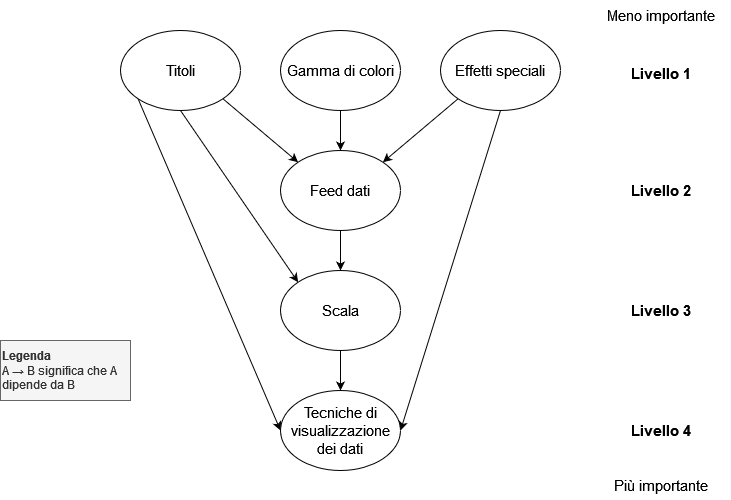
\includegraphics[width=0.8\columnwidth]{infografiche/fattori_design_info.png} 
    \caption{Gerarchia dei fattori che influenzano il design delle infografiche}
    \label{fig:fattori_design_info}
\end{figure}
\noindent Vediamo dunque come applicare al meglio tali fattori nella costruzione del design di un'infografica.

\subsubsection{I colori}
%“Design della mente – infografica e data viz” di Paolo Bottazini, Michele Gotuzzo
%CAP 16: Il colore
Il colore è un elemento cruciale nel design delle infografiche e, pertanto, è da utilizzare con cura. 
Esso infatti, se scelto in maniera appropriata, può migliorare la leggibilità e facilitare la comprensione e memorizzazione dell'informazione.

Generalmente, si utilizza il colore per catturare l'attenzione, evidenziare dati specifici e per rafforzare il messaggio narrativo. Quest'ultimo punto, in particolare, è possibile in quanto ogni colore porta con sé un 
significato simbolico influenzato dalla cultura e dalla geografia che permette di evocare sensazioni e valori specifici nel pubblico.
Di seguito sono riportati i valori più spesso associati ai colori, con riferimento alla cultura dell'Occidente:
\begin{itemize}
    \item Colori caldi:
    \begin{itemize}
        \item \textbf{Rosso}:
        \begin{itemize}
            \item Valori: emozioni forti come amore o aggressività.
            \item In linea con tali valori, viene utilizzato principalmente per attirare l'attenzione.
        \end{itemize}
        \item \textbf{Arancione}:
        \begin{itemize}
            \item Valori: ottimismo, vitalità.
            \item In linea con tali valori, viene generalmente utilizzato per temi giovanili e/o dinamici.
        \end{itemize}
        \item \textbf{Giallo}:
        \begin{itemize}
            \item Valori: energia, allegria, felicità.
            \item In linea con tali valori, viene anch'esso utilizzato principalmente per attirare l'attenzione, specie per temi innovativi.
        \end{itemize}
    \end{itemize}
    \item Colori freddi:
    \begin{itemize}
        \item \textbf{Verde}:
        \begin{itemize}
            \item Valori: salute, natura, tranquillità.
            \item In linea con tali valori, viene generalmente utilizzato per temi riguardanti la sanità, salute ed ecologia.
        \end{itemize}
        \item \textbf{Blu}:
        \begin{itemize}
            \item Valori: affidabilità, sicurezza, stabilità.
            \item In linea con tali valori, viene utilizzato ad esempio da banche o compagnie assicurative.
        \end{itemize}
        \item \textbf{Viola}:
        \begin{itemize}
            \item Valori: eleganza, nobiltà, spiritualità.
            \item In linea con tali valori, viene generalmente utilizzato per temi riguardanti il settore della bellezza o del lusso.
        \end{itemize}
    \end{itemize}
    \item Colori neutri:
    \begin{itemize}
        \item \textbf{Marrone}:
        \begin{itemize}
            \item Valori: terra, calore.
            \item In linea con tali valori, viene generalmente utilizzato per temi riguardanti la natura.
        \end{itemize}
        \item \textbf{Bianco}:
        \begin{itemize}
            \item Valori: purezza, pulizia, semplicità.
            \item In linea con tali valori, viene generalmente utilizzato per temi riguardanti la sanità.
        \end{itemize}
        \item \textbf{Nero}:
        \begin{itemize}
            \item Valori: ribellione, formalità, potenza.
            \item In linea con tali valori, viene generalmente utilizzato per temi di protesta o riguardanti il settore del lusso.
        \end{itemize}
        \item \textbf{Grigio}:
        \begin{itemize}
            \item Valori: modernità, raffinatezza.
            \item In linea con tali valori, viene generalmente utilizzati per temi riguardanti tecnologia o moda.
        \end{itemize}
    \end{itemize}
\end{itemize}

\bigskip
\noindent In ogni caso, è fondamentale mantenere un tono di colore coerente nell'infografica, preferibilmente tonalità sobrie. Tuttavia, potrebbe essere utile adoperare colori 
complementari per trasmettere sensazioni di calma oppure combinazioni di colori più stridenti per rappresentare innovazione.

Si aggiunge infine che, come per la \gls{datavizg}, anche in questo caso, è importante scegliere una gamma di colori che sia accessibile anche a persone daltoniche o \emph{color-deficient}.

\subsubsection{I layout}\label{subsec:info_layout}
% “Visual doing” di Willemien Brand 
Gli elementi di un'infografica possono essere disposti in un massimo di sei livelli:
\begin{itemize}
    \item Il \textbf{titolo principale};
    \item Il \textbf{sottotitolo};
    \item Il \textbf{contenuto principale e secondario};
    \item Gli \textbf{elementi di supporto}, come ad esempio divisori, contenitori etc.
    \item Gli \textbf{elementi di dettaglio}, come ad esempio le note a margine;
    \item I \textbf{comandi} di interazione e gli \textbf{\emph{highlights}} dei dati.
\end{itemize}

\bigskip
% Acquired Codes of Meaning in Data Visualization and Infographics: Beyond Perceptual Primitives, Lydia Byrne, Daniel Angus, and Janet Wiles
\noindent Per quanto riguarda nello specifico la struttura del contenuto principale e secondario, le infografiche sono solite
utilizzare una ``composizione a \emph{panel}'', ovvero si hanno diverse componenti grafiche, dette \emph{gruppi visivi}, leggibili in sequenza.
Questo approccio differisce notevolmente dalle pratiche comunemente usate nella \gls{datavizg}, dove tutte le sfaccettature del tema d'interesse sono presentate 
in un'unica composizione grafica.

La direzione e ordine in cui questa sequenza di \emph{gruppi visivi} viene presentata all'interno dell'infografica dipende dalla 
storia che si vuole raccontare. Infatti, per trasmettere efficacemente le informazioni e la narrativa, è necessario avere una struttura semantica sottostante all'infografica
che collega i \emph{gruppi visivi} in una determinata maniera dipendente dal messaggio. Questa struttura è detta \gls{vif}, letteralmente ``flusso delle informazioni visive''.
Tale flusso è spesso rimarcato ed evidenziato tramite l'uso di ``suggerimenti narrativi'', che possono essere espliciti, come frecce o descrizione testuali, oppure impliciti, se 
provengono da vari principi di design come ad esempio i principi di \emph{Gestalt} (approfonditi alla sezione \ref{subsec:gestalt}).
%TODO: studi di ... che analizzano vif nei vari hanno permesso di individuare pattern

Sono individuati i seguenti \emph{pattern} principali di \gls{vif}, distinti in base alla loro \emph{backbone shape}, ovvero da una diversa forma della linea lungo cui la 
maggior parte dei \emph{gruppi visivi} è allineata nella narrazione.
\begin{table}[H]
    \centering
    %\begin{tabular}{|m{0.12\textwidth}|m{0.30\textwidth}|m{0.12\textwidth}|m{0.30\textwidth}|}
    \begin{tabular}{|>{\centering\arraybackslash} m{0.15\textwidth}| >{\centering\arraybackslash} m{0.3\textwidth}| >{\centering\arraybackslash} m{0.15\textwidth}| >{\centering\arraybackslash} m{0.3\textwidth}|}
        \hline
        \rowcolor{gray!30}
        \textbf{Backbone Shape} & \textbf{Pattern} & \textbf{Backbone Shape} & \textbf{Pattern} \\
        \hline
        \begin{center}
\includegraphics[width=0.08\textwidth]{infografiche/clock_vif.png}\end{center} & Clock 
        & \begin{center}
\includegraphics[width=0.08\textwidth]{infografiche/downladder_vif.png}\end{center} & Down-ladder \\
        \begin{center}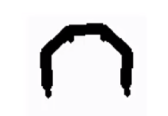
\includegraphics[width=0.08\textwidth]{infografiche/dome_vif.png}\end{center} & Dome
        & \begin{center}
\includegraphics[width=0.08\textwidth]{infografiche/upladder_vif.png}\end{center} & Up-ladder \\
        \begin{center}
\includegraphics[width=0.08\textwidth]{infografiche/bowl_vif.png}\end{center} & Bowl
        & \begin{center}
\includegraphics[width=0.08\textwidth]{infografiche/landscape_vif.png}\end{center} & Landscape \\
        \begin{center}
\includegraphics[width=0.08\textwidth]{infografiche/leftwing_vif.png}\end{center} & Left-wing 
        & \begin{center}
\includegraphics[width=0.08\textwidth]{infografiche/portrait_vif.png}\end{center} & Portrait \\
        \begin{center}
\includegraphics[width=0.08\textwidth]{infografiche/rightwing_vif.png}\end{center} & Right-wing
        & \begin{center}
\includegraphics[width=0.08\textwidth]{infografiche/pulse_vif.png}\end{center} & Pulse \\
        \begin{center}
\includegraphics[width=0.08\textwidth]{infografiche/star_vif.png}\end{center} & Star 
        & \begin{center}
\includegraphics[width=0.08\textwidth]{infografiche/spiral_vif.png}\end{center} & Spiral \\
        \hline
    \end{tabular}
    \vspace{0.2cm}
    \caption{Backbone shape dei pattern di Visual Information Flow (VIF)}
    \label{tab:pattern_vif}
\end{table}

\noindent Le informazioni, dunque, saranno disposte all'interno dell'infografica a seconda dell'obiettivo della storia da raccontare.
Per la definizione degli obiettivi si rimanda alla sezione \ref{subsec:info_classifica}.

Nello specifico, vengono definite le seguenti disposizioni generali a cui si possono facilmente far corrispondere i diversi \emph{pattern} di \gls{vif} sopraelencati. 
% “Visual thinking” di Willemien Brand 
\begin{itemize}
    \item Disposizione \textbf{a lista}:
    \begin{itemize}
        \item Applicazione: come suggerisce il nome è adatta a infografiche che hanno come obiettivo rappresentare un elenco (e.g. orari o programmi), ma 
        anche infografiche basate su una gerarchia.
        \item Direzione: la storia viene presentata a partire dall'alto verso il basso. In alcuni casi, potrebbe anche essere orientata da sinistra verso destra.
        \item \emph{Pattern} \gls{vif}:
        \begin{itemize}
            \item \textbf{Portrait};
            \item \textbf{Landscape};
            \item \textbf{Down-ladder}. 
        \end{itemize}
    \end{itemize}
    \item Disposizione \textbf{a passi}:
    \begin{itemize}
        \item Applicazione: per infografiche che rappresentano processi ordinati.
        \item Direzione: la storia viene presentata dal basso verso l'alto e/o seguendo un percorso a zigzag che parte da sinistra e, generalmente, termina al lato opposto.
        \item \emph{Pattern} \gls{vif}:
        \begin{itemize}
            \item \textbf{Pulse};
            \item \textbf{Spiral};
            \item \textbf{Up-ladder}. 
        \end{itemize}
    \end{itemize}
    \item \textbf{\emph{Timeline}}:
    \begin{itemize}
        \item Applicazione: per infografiche basate sul tempo.
        \item Direzione: la storia viene presentata da sinistra verso destra oppure dall'alto verso il basso, solitamente avendo come riferimento una singola linea rappresentante il tempo.
        \item \emph{Pattern} \gls{vif}:
        \begin{itemize}
            \item \textbf{Portrait};
            \item \textbf{Landscape}.
        \end{itemize}
    \end{itemize}
    \item Disposizione \textbf{a mandala}:
    \begin{itemize}
        \item Applicazione: per infografiche basate su informazioni correlate poste allo stesso livello.
        \item Direzione: la storia si sviluppa dal centro verso l'esterno, seguendo un \emph{pattern} radiale che si estende nelle quattro direzioni diagonali o, più in generale, verso tutti i lati in modo sistematico.
        \item \emph{Pattern} \gls{vif}:
        \begin{itemize}
            \item \textbf{Clock};
            \item \textbf{Star};
            \item Variazioni dei modelli suddetti, come: \textbf{dome}, \textbf{bowl}, \textbf{left-wing} e \textbf{right-wing}.
        \end{itemize}
    \end{itemize}
    \item Disposizione a \textbf{matrice e divisa in due}:
    \begin{itemize}
        \item Applicazione: per infografiche basate sul confronto.
        \item Direzione: in caso di confronto tra due elementi lo spazio viene diviso verticalmente in due, mentre in caso di quattro si ha una suddivisione data dai quattro angoli, a formare una sorta di piano cartesiano.
        \item \emph{Pattern} \gls{vif}:
        \begin{itemize}
            \item \textbf{Clock}.
        \end{itemize}
    \end{itemize}
\end{itemize}
Si noti che i \emph{pattern} \gls{vif} potrebbero essere applicati in maniera composita per diverse macro-aree dell'infografica.

\subsubsection{La grandezza degli elementi}
La scelta della dimensione degli elementi deve essere fatta con cura per poter garantire l'accessibilità dei dati, una simmetria nel design e poter trasmettere correttamente l'ordine di importanza 
dei dati presentati.

Innanzitutto, è essenziale che tutti gli elementi abbiano dimensioni sufficienti a essere visti e/o letti agevolmente. Ciò è particolarmente importante per infografiche web destinate alla visualizzazione su schermi con
dimensioni diverse, come computer e dispositivi mobili.

In secondo luogo, gli elementi e dati più rilevanti dovrebbero avere dimensioni maggiori per poter attirare l'attenzione del lettore, mentre i dettagli secondari possono essere più piccoli.
La scala degli elementi è importante dunque anche per dare una sorta di ``gerarchia visiva'', che permette di strutturare meglio l'infografica, facilitando il confronto tra elementi con stesso livello ed evidenziando sezioni e 
relazioni tra le parti.

\subsubsection{Le tecniche di visualizzazione dei dati inserite}
Un elemento determinante nella presentazione dei dati nelle infografiche è rappresentato dalle tecniche di \gls{datavizg} utilizzate e, nello specifico, dalla scelta dei grafici e diagrammi.
Questo argomento è già stato affrontato nella sezione \ref{sec:classificare_grafici}, che riguarda la classificazione dei grafici e la loro scelta tramite lo strumento \emph{Chart-chooser}.

\subsubsection{La simmetria nel design}
La simmetria è un altro principio fondamentale nel design delle infografiche, poiché contribuisce a creare un senso di equilibrio e ordine visivo che può aiutare l'occhio del lettore a orientarsi
all'interno dell'infografica.

Tale equilibrio può essere raggiunto in due diversi modi:
\begin{itemize}
    \item \textbf{\emph{Symmetrical balance}}: si distribuiscono gli elementi in modo simmetrico rispetto a un asse centrale, orizzontale o rispetto a un punto centrale. L'obiettivo è creare una composizione visivamente stabile, elegante e prevedibile.
    Tale approccio porta a creare infografiche con \emph{layout} molto strutturati e ordinati.
    \begin{itemize}
        \item Tale metodo è visibile nella maggior parte dei \emph{pattern} \gls{vif}, come ad esempio \emph{portrait} (asse orizzontale), \emph{landscape} (asse verticale) o \emph{layout} circolari (attorno a punto centrale).
    \end{itemize}
    \item \textbf{\emph{Asymmetrical balance}}: si accetta un certo livello di asimmetria e dinamicità nel \emph{layout} dell'infografica, pur mantenendo una sensazione generale di equilibrio visivo. In questo approccio, la scelta di proporzioni e distribuzione
    degli elementi è più flessibile, tuttavia si pone comunque una particolare attenzione a evitare la presenza di parti nell'infografica che appaiano troppo pesanti o trascurate.
    \begin{itemize}
        \item Esistono modelli \gls{vif}, come \emph{up-ladder} e \emph{down-ladder}, dove gli elementi sono decentrati e posizionati sul lato opposto del titolo per mantenere l'equilibrio.
    \end{itemize}
\end{itemize}


\subsubsection{Gli elementi grafici}
Oltre a grafici, diagrammi ed elementi testuali, l'infografica può contenere anche altre tecniche di comunicazione visiva. Tra queste, ad esempio, vengono spesso utilizzati
illustrazioni, icone e simboli.

%“Design della mente – infografica e data viz” di Paolo Bottazini, Michele Gotuzzo
%CAP 18: Le immagini
Tali tecniche consentono di facilitare la memorizzazione, grazie alla loro potenza evocativa e alla loro capacità di richiamare oggetti facilmente riconoscibili dall'uomo.

\bigskip
\noindent Alcune linee guida da seguire per ottimizzarne l'uso, e costruire così una comunicazione efficace, sono:
\begin{itemize}
    \item Seguire i \textbf{principi di \emph{Gestalt}} (meglio approfonditi alla sezione \ref{subsec:gestalt});
    \item \textbf{Selezionare immagini evocative} che possano provocare un'esperienza sensoriale all'utente;
    \item Fare particolare \textbf{attenzione alla risoluzione dell'immagine} in modo che questa sia sempre visibile e nitida.
\end{itemize}

\subsubsection{I blocchi di testo}
È bene ricordare che l'infografica non è lo strumento perfetto per ogni situazione. L'infografica, infatti, è utile solo quando si dispone di sufficienti informazioni 
per raccontare una storia, senza però eccedere. Un testo troppo lungo può creare ``rumore'' e compromettere l'efficacia della comunicazione.

Generalmente i blocchi di testo presenti in un'infografica sono:
\begin{itemize}
    \item Il \textbf{titolo};
    \item Il \textbf{sottotitolo}, che specifica i contenuti annunciati con il titolo, pertanto non può esistere senza quest'ultimo;
    \item L'\textbf{introduzione}, inserita solitamente vicino a titolo e posta in corsivo, specifica ulteriormente il tema dell'infografica e funge da ``guida'' per la sua lettura;
    \item Il \textbf{testo principale}, che serve a spiegare meglio le informazioni visualizzate con altri mezzi (e.g. grafici);
    \item Le \textbf{note a piè di pagina}, che servono a dare informazioni a carattere formale (e.g. fonti) all'utente e dunque utilizzano il più piccolo carattere leggibile possibile per evitare 
    di distrarlo.
\end{itemize}
Tra questi, la parte forse più importante degli elementi testuali di un'infografica sono i titoli (sia quello globale sia quelli, seppur in minor misura, dei singoli blocchi).
Le intestazioni devono, infatti, essere incisive e invogliare il fruitore dell'infografica a continuare a visionare la presentazione. 
A tal fine, i titoli sono generalmente formulati in uno dei seguenti modi:
\begin{itemize}
    \item \textbf{Sotto forma di domanda}, si pone un interrogativo curioso o interessante che stimoli il lettore a cercarne la risposta nei dati presentati.
    \item \textbf{Includendo la statistica principale}, evidenziando il dato presentato più significativo.
    \item \textbf{Come confronto}, si mette in relazione fin da subito due o più elementi di cui se ne mostreranno differenze e similitudini.
    \item \textbf{Come introduzione a un elenco numerato}, il titolo funziona come introduzione a una lista (e.g. ``Top X'').
\end{itemize}

\subsubsection{I caratteri tipografici}
%“Design della mente – infografica e data viz” di Paolo Bottazini, Michele Gotuzzo
%CAP 17: I caratteri
L'elemento più importante nel design di un'infografica è la scelta del carattere tipografico, il quale influisce pesantemente sulla leggibilità e comprensibilità dell'infografica. 
Nello specifico, la gamma di caratteri utilizzati non deve essere troppo amplia (max. 3 o 4); bisogna invece concentrarsi sulla scelta del tipo di carattere, il quale
può avere un impatto significativo sul design complessivo dell'infografica.

A tal fine, si possono applicare le seguenti regole:
\begin{itemize}
    \item Per quanto riguarda l'uso di \textbf{caratteri graziati} (\emph{serif}), essi sono da utilizzare quando si vuole conferire serietà e autorevolezza al testo; sono infatti impiegati tipicamente in saggi e quotidiani. 
    Tuttavia, possono risultare meno leggibili su schermo.
    \begin{itemize}
        \item Esempio: Times New Roman.
    \end{itemize}
    \item Per quanto riguarda l'uso di \textbf{caratteri senza grazie} (\emph{sans serif}), essi sono da utilizzare per testi brevi e/o su schermi, in quanto più leggibili.
    \begin{itemize}
        \item Esempio: Arial (adatto per testi lunghi, essendo più stretto), Verdana (ideale per frasi ad effetto), Helvetica.
    \end{itemize}
    \item Per quanto riguarda l'uso di \textbf{caratteri decorativi}, essi sono spesso difficili da utilizzare e generalmente, dunque, sono da evitare. Possono essere considerati, seppur con prudenza, per casi specifici per riflettere il tema discusso nella presentazione.
    \begin{itemize}
        \item Esempio: caratteri calligrafici o fumettistici.
    \end{itemize}
    \item Per quanto riguarda l'uso del \textbf{grassetto} (\emph{bold}), è da utilizzare per evidenziare componenti testuali brevi e focalizzare l'attenzione su di essi. 
    \item Per quanto riguarda l'uso del \textbf{corsivo} (\emph{italic}), è da utilizzare per citazioni o termini particolari.
    \item Per quanto riguarda l'uso del \textbf{maiuscolo}, è da utilizzare per dare maggiore importanza o evidenziare testi brevi, come i titoli, in quanto corrisponde ad un ``innalzamento della voce''.
\end{itemize}
Sempre con riferimento ai caratteri, è importante seguire anche le seguenti regole:
\begin{itemize}
    \item Per quanto riguarda la \textbf{sottolineatura}, nel web questa è da evitare per evidenziare elementi (preferendo invece il grassetto), in quanto solitamente rappresenta un collegamento 
    ipertestuale.
    \item Per quanto riguarda l'\textbf{interlinea}, conviene che la distanza tra una riga e l'altra sia abbastanza ampia da consentire una lettura agevole.
    \item Per quanto riguarda l'\textbf{allineamento}, si utilizza solitamente il ``centrato'' per i titoli, specie se non accompagnati da ulteriore testo. Per il resto, si preferisce invece l'allineamento
    ``a sinistra''.
    \item Per quanto riguarda la \textbf{lunghezza}, testi troppo lunghi non sono letti volentieri dal pubblico e, inoltre, necessiterebbero di caratteri più piccoli, meno leggibili.
\end{itemize}


\subsection{Interattività}
%intro: “L'arte funzionale – Infografica e visualizzazione delle informazioni” di Alberto Cairo
% cap 9
%TODO: footnote Principio delle informazioni visive di Ben Schneiderman
Per quanto riguarda la navigazione ed esplorazione delle infografiche si applica generalmente il cosiddetto \textbf{principio delle informazioni visive}, che afferma:
``prima panoramica, zoom e filtri, poi dettagli su richiesta''. Si devono dunque presentare i punti salienti e più rilevanti, mentre ulteriori informazioni sono fornite agli utenti solo con il loro addentrarsi ed esplorazione
minuziosa dell'infografica. 

Le tecniche di esplorazione e navigazione possibili sono le seguenti:
\begin{itemize}
    \item \textbf{Scorrimento e \emph{panning}}, il primo utilizzato generalmente su siti web con orientamento verticale, mentre il secondo solitamente viene usato su mappe per spostarsi;
    \item \textbf{Zoom}, anch'esso da usare ad esempio su mappe;
    \item \textbf{Apertura e chiusura}, ad esempio per aprire o chiudere finestre \emph{pop-up} di dettaglio;
    \item \textbf{Classificazione e riordino}, ad esempio riordinando i dati contenuti su una tabella;
    \item \textbf{Ricerca e filtro}.
\end{itemize}
L'utente può impiegare tali tecniche interagendo con l'interfaccia nei seguenti modi:
\begin{itemize}
    \item \textbf{Tramite istruzioni}, l'utente dà un input diretto all'infografica (e.g. cliccando un pulsante), la quale si adatta di conseguenza;
    \item \textbf{Tramite dialogo}, l'utente ``dialoga'' con la presentazione (e.g. ad esempio tramite finestre di dialogo) e ne cambia, in tal modo, i parametri;
    \item \textbf{Manipolazione}, l'utente cambia la struttura o l'aspetto della visualizzazione (e.g. tramite filtraggio dei dati rappresentati);
    \item \textbf{Esplorazione}, l'utente ha la sensazione di star dirigendo in prima persona l'azione (e.g. muovendosi all'interno di modelli 3D).
\end{itemize}

\bigskip
\noindent Applicare queste tecniche aiuta a rendere la presentazione dei dati più coinvolgente e chiara, contribuendo così a raggiungere meglio gli obiettivi delle infografiche.
Tuttavia, per un loro giusto impiego, è necessario seguire questi principi:
%TODO: citazione “The design of everyday things” di Donald A. Norman ? che tratta di come ci rapportiamo a oggetti comuni. 
% Priorità è sui bisogni dell'utente rispetto alle preoccupazioni estetiche dei designer
\begin{itemize}
    \item \textbf{Visibilità}, ossia rendere il più visibile la funzionalità di un oggetto in modo che sia più facile per gli utenti riconoscerlo e capirne la funzionalità. Tale norma può
    essere implementata tramite la forma dell'oggetto, che spesso suggerisce visivamente la funzionalità che esso permette (e.g. pulsante sul web che somigli a uno reale), oppure semplicemente tramite
    la mera organizzazione degli elementi visivi. Infatti, se un'informazione è fondamentale per la comprensione dell'intera infografica, essa dovrebbe essere sempre visibile e non nascosta da uno strato di interattività.
    \item \textbf{Feedback}, ciò significa che a ogni azione dell'utente si dovrebbe avere una reazione che indichi l'esito dell'operazione.
    \item \textbf{Vincoli}, ovvero devono essere posti dei vincoli in modo da orientare la navigazione dell'utente.
    \item \textbf{Uniformità}, ciò implica che entità analoghe dovrebbero somigliarsi.
\end{itemize}


\subsection{Principi di Gestalt}\label{subsec:gestalt}
%intro: “L'arte funzionale – Infografica e visualizzazione delle informazioni” di Alberto Cairo
% cap 6
La \emph{Gestalt} (letteralmente ``forma'' o ``schema'' in tedesco) è una corrente psicologica che analizza e studia il funzionamento del cervello umano per cercare di prevedere come questo percepisce e organizza le informazioni visive. 
Nello specifico, i principi definiti da questa psicologia si basano sulla capacità del cervello di riconoscere schemi e classificare elementi visivi basandosi su differenze e somiglianze, anche prima che venga prestata attenzione consapevole ai dettagli specifici (si parla, infatti, di ``percezione pre-attentiva''). 
Per tali motivi, incorporare questi concetti nella progettazione delle infografiche potrebbe migliorare l'efficacia comunicativa e, al contempo, rendere l'interfaccia grafica più intuitiva per l'utente.

%“Design della mente – infografica e data viz” di Paolo Bottazini, Michele Gotuzzo
%CAP 15: Gestalt (parte di design) 
%Design is storytelling” di Ellen Lupton
%atto 3
Vediamo dunque come applicare le leggi di \emph{Gestalt} al caso specifico del design di infografiche:
\begin{itemize}
    \item \textbf{Legge di pregnanza}, siccome il cervello umano tende a elaborare i \emph{pattern} regolari e ordinati più velocemente, si organizzino i dati logicamente e in maniera semplice. 
    Si tenga inoltre conto che, sempre per questo principio, se si hanno linee o forme regolari con degli spazi, questi vengono mentalmente chiusi.    
    \item \textbf{Legge di continuità} (di direzione), siccome il cervello umano tende a raggruppare oggetti vicini o allineati, si organizzino i dati di uno stesso gruppo concettuale vicini tra loro e con uno stesso allineamento. 
    Tale configurazione permette di facilitare il processo di raggruppamento, comparazione e conseguente comprensione da parte dell'utente.     
    \item \textbf{Legge di similarità}, siccome elementi con caratteristiche simili (e.g. colore, forma, dimensione, orientamento) vengono percepiti come un unico gruppo, si utilizzino caratteristiche simili per stabilire relazioni tra i vari elementi.
    \item \textbf{Legge del punto focale}, simmetricamente alla legge precedente, si utilizzino caratteristiche diverse per aumentare il divario tra i vari gruppi ed evidenziare i punti salienti, creando punti focali che attirino l'attenzione dell'utente. 
    \item \textbf{Legge degli isomorfi}, siccome gli eventi e gli elementi sono interpretati dagli utenti in base alla loro esperienza passata, si tenga conto dei condizionamenti dati da cultura e dalle abitudini e convenzioni adottate.
    \item \textbf{Legge dell'immagine e dello sfondo}, siccome gli elementi vengono interpretati in maniera diversa in base alle relazioni con lo sfondo, si assicuri di avere un grande contrasto tra le informazioni e lo sfondo se le prime sono molto importanti, mentre si possono integrare dati nello sfondo se questi non particolarmente rilevanti. 
    \item \textbf{Legge del fato o del destino comune}, siccome un gruppo di elementi simili è percepito come una struttura strettamente correlata, si utilizzino orientamenti, direzioni o movimenti per stabilire o interrompere le relazioni tra i componenti.
\end{itemize}



\section{Come costruire un'infografica}
%“Design della mente – infografica e data viz” di Paolo Bottazini, Michele Gotuzzo 
\subsection{L'Infomodel}
%CAP 6: Uno sguardo sul piano di lavoro (INFOMODEL)
%TODO: inserire footnote fonte
Per garantire un prodotto finale di comunicazione efficace, la progettazione di un'infografica deve seguire un preciso schema, detto \emph{Infomodel}. 
Nello specifico, questo modello si compone di una serie ordinata di passaggi:
\begin{enumerate}
    \item \textbf{Identificazione degli interlocutori};
    \item \textbf{Identificazione della storia e dei suoi effetti};
    \item \textbf{Identificazione del \emph{dataset}};
    \item \textbf{Analisi dei dati};
    \item \textbf{Rappresentazione della storia}.
\end{enumerate}
Si approfondiscono tali passaggi nei paragrafi successivi.

\subsubsection{Identificazione degli interlocutori}
%CAP 7: Identificare il tipo di pubblico (infomodel 1)
L'obiettivo dell'infografica è rappresentare l'argomento secondo le preferenze degli interlocutori. Nello specifico, si vogliono presentare le informazioni 
rispecchiando le inclinazioni cognitive e decisionali della maggior parte del pubblico sul tema.

A tal fine, è possibile formulare un modello di classificazione decisionale che ha come obiettivo l'adeguamento al pubblico della narrazione sul piano pragmatico,
che consideri dunque le persuasioni e azioni che l'enunciazione delle frasi comporta. 

\paragraph{Inclinazioni cognitive.}
Quando parliamo di ``inclinazioni cognitive'' intendiamo, generalmente, le modalità di comprensione e di analisi dei fenomeni.
Tali inclinazioni possono essere riassunte con il \gls{mbti}, strumento che divide le preferenze degli utenti in quattro coppie di 
opposti. Tali coppie sono:
\begin{itemize}
    \item \textbf{Estroversione o Introversione}, fornisce una preferenza riguardante il modo di trarre energia dell'individuo.
    Se ci si concentra più sul mondo esterno che quello interiore si tende al primo valore, in caso contrario al secondo.   
    \item \textbf{Sensitività o Intuizione}, fornisce una preferenza riguardante la modalità di acquisire informazioni. 
    Se ci si concentra più sui fatti concreti che sul quadro generale e sulle possibili implicazioni si tende al primo valore, in caso contrario al secondo.
    \item \textbf{Ragionamento o Sentimento}, fornisce una preferenza sulle modalità di decisione e raggiungimento di conclusioni.
    Se si adotta un approccio più oggettivo che empatico si tende al primo valore, in caso contrario al secondo.
    \item \textbf{Giudicare o Percepire}, fornisce preferenza sui modi di rapportarsi con il mondo esterno.
    Se non si è flessibili e non si è aperti a nuove informazioni si tende al primo valore, in caso contrario al secondo.
\end{itemize}
Ogni individuo tende a preferire uno dei due valori di ciascuna coppia. La combinazione di queste preferenze corrisponde a un tipo di personalità, il quale influenza l'approccio
dell'individuo alla comprensione e all'analisi delle informazioni. Infatti, ciascun diverso tipo si comporta diversamente e ha differenti interessi, opinioni e motivazioni. 
Pertanto, la consapevolezza delle differenze tra i tipi può aiutare a strutturare l'infografica in modo più efficace.
%TODO: inserire immagine?

\paragraph{Inclinazioni decisionali.}
Quando parliamo invece di ``inclinazioni decisionali'' intendiamo le modalità di apprendimento con cui un individuo riesce ad arrivare più facilmente alla \emph{saggezza}. 
Tali inclinazioni possono essere riassunte con il modello \emph{\textbf{4MAT}} sviluppato da Bernice McCarthy, il quale individua quattro diversi stili di apprendimento basati 
sulle domande che gli individui si pongono riguardo al contenuto del materiale di studio. A ciascun stile è dunque facilmente associabile una modalità di narrazione che si concentra
sul rispondere a tali domande.
Questi stili sono:
\begin{enumerate}
    \item \textbf{Apprendimento ``innovativo''}
    \begin{itemize}
        \item Principale interrogativo: ``perchè?''
        \item Tipo di individui: comprende tutte le persone che tendono a interrogarsi e riflettere sulla rilevanza e importanza concreta di un argomento prima di affrontarlo.
        Essi vogliono sapere il significato e i motivi per cui un fatto è accaduto.
        \item Tipo di narrazione: la spiegazione, in quanto racconta il significato e le ragioni.
    \end{itemize}
    \item \textbf{Apprendimento ``analitico''}
    \begin{itemize}
        \item Principale interrogativo: ``cosa?''
        \item Tipo di individui: comprende tutte le persone che tendono a raccogliere fatti per approfondire la loro conoscenza dell'argometno. Essi vogliono
        dunque saperne il più possibile di un determinato concetto e analizzarlo in dettaglio.
        \item Tipo di narrazione: una descrizione più completa possibile della questione che fornisca tutti gli attori della storia.
    \end{itemize}
    \item \textbf{Apprendimento basato sul ``buonsenso''}
    \begin{itemize}
        \item Principale interrogativo: ``come?''
        \item Tipo di individui: comprende tutte le persone che preferiscono sperimentare e mettere in pratica prima di formarsi una piena opinione in merito all'argomento. Essi vogliono
        dunque capire come possono utilizzare le informazioni per poter migliorare le proprie competenze.
        \item Tipo di narrazione: un racconto che svisceri il modo in cui si svolge il processo descritto, specificando requisiti, dettagli e attori in gioco.
    \end{itemize}
    \item \textbf{Apprendimento ``dinamico''}
    \begin{itemize}
        \item Principale interrogativo: ``cosa succede se?''
        \item Tipo di individui: comprende tutte le persone il cui apprendimento è dato da una scoperta autonoma dettata dalla propria intuizione.
        Essi sono dunque interessati a capire le possibili conseguenze future e applicazioni pratiche delle diverse situazioni per adattarsi ai cambiamenti nell'ambiente o alle nuove possibilità che queste potrebbero comportare.
        \item Tipo di narrazione: una storia che esplora e incorpora tutte le opzioni e possibilità derivanti dalle scelte presentate.
    \end{itemize}
\end{enumerate}
%TODO: inserire immagine?
Per un apprendimento accessibile a tutti, il \emph{4MAT} prevede la combinazione di questi stili nell'ordine presentato sopra. Nello specifico, si dovrebbe iniziare con una spiegazione del perché l'argomento è rilevante e perché il pubblico dovrebbe
essere interessato ad ascoltarlo, seguito da una descrizione dettagliata e oggettiva dei dati e delle informazioni in merito, proseguendo con un'esplorazione dei risvolti pratici di quanto specificato e concludendo con una panoramica delle possibili 
conseguenze e cambiamenti futuri. 

Tuttavia, per ottimizzare ulteriormente la comunicazione, è importante adattare la narrazione al tipo di pubblico specifico, approfondendo maggiormente la parte dettata dallo stile predominante tra gli interlocutori.
Ciò consente di raggiungere una maggiore efficacia del messaggio e facilitarne una comprensione più profonda da parte del pubblico.

\subsubsection{Identificazione della storia e dei suoi effetti}
\paragraph{Formulare una storia.}
%CAP 8: Formulare la storia (infomodel 2)
Essenziale per una buona infografica è l'individuazione di una narrativa coinvolgente.
A tal fine, si utilizza la struttura classica del racconto, ovvero un arco narrativo sviluppato in tre atti come segue:
\begin{itemize}
    \item \textbf{Inizio}: presentazione dell'equilibrio iniziale e della sua rottura. Viene fornita una panoramica dello stato dell'arte dell'argomento e si mostrano gli agenti coinvolti. 
    Successivamente si espongono il motivo o la complicazione che spinge verso il cambiamento, solitamente sotto forma di domanda.
    \item \textbf{Sviluppo}: esplorazione delle ``peripezie'' degli agenti coinvolti, ovvero vengono esposte le azioni compiute che cercano di rispondere alla domanda iniziale.
    Questo atto comporta dunque la crescita dell'azione, il suo climax e termina con la decrescita dell'azione stessa. È importante che questo processo non sia troppo affrettato: 
    se la risposta alla domanda iniziale è fornita troppo presto, la storia rischia di diventare noiosa o banale.
    \item \textbf{Conclusione}: ripristino dell'equilibrio attraverso le azioni svolte dagli agenti, si torna dunque a una nuova stabilità che costituisce l'epilogo della storia.
\end{itemize} 

\bigskip
%Design is storytelling” di Ellen Lupton
%ATTO 1: \emph{pattern} storie (pianificazione dello scenario)
\noindent Da tale descrizione, possiamo dunque identificare i principali elementi di una storia in agenti e azioni. Gli agenti sono i soggetti o le forze che influiscono o vengono influenzati dai dati, mentre 
le azioni sono gli eventi o le decisioni che modellano la storia stessa. Si noti, inoltre, che quest'ultime devono seguire i seguenti criteri:
\begin{itemize}
    \item trasformare gli agenti o la situazione, ogni azione deve dunque generare un \textbf{cambiamento};
    \item trasmettere un significato, ogni azione è dunque collegata a un \textbf{tema};
    \item basarsi su dettagli rilevanti, ogni azione è dunque compiuta con \textbf{coerenza};
    \item seguire delle regole ed essere credibili, ogni azione deve dunque rispettare il principio di \textbf{plausibilità}.
\end{itemize}

\paragraph{Gli effetti della storia.} 
%ATTO 2: esprimere emozioni
È cruciale considerare non solo l'esperienza utente dell'infografica al momento dell'interazione, ma anche come tale esperienza sarà ricordata dall'utente in futuro.
Diventa dunque necessario empatizzare con i valori e le aspirazioni del pubblico per poter realizzare un design che provochi reazioni istantanee, siano esse viscerali (come risposta a colori, materiali etc.) o fisiche (e.g. cliccare un pulsante), e che al contempo
innesti memorie e associazioni permanenti relative all'infografica.

\bigskip
\noindent Dal punto di vista pratico, tale processo può essere realizzato creando degli archetipi di utenti che aiutino a comprendere come persone con diversi desideri e abilità potrebbero approcciarsi all'infografica. 
A tal fine, si noti che è particolarmente importante ricostruire quale siano storia, emozioni, risorse e obiettivi di queste ``persone'' in modo tale da poter capire il perché di alcune loro azioni. Meno interessante, invece, è individuare
quale siano le singole azioni effettuate.

\subsubsection{Identificazione del dataset}
%CAP 9: Individuare il dataset (infomodel 3)
Si scelgono dei \emph{dataset} in base ai punti precedenti e facendo attenzione all'autorevolezza delle fonti e alla rappresentatività del campione.
Successivamente, è necessario pulire i dati per renderli coerenti con le convenzioni adottate globalmente e per sostituire eventuali incoerenze di notazione con le corrette.

A seconda dei dati disponibili scelti, si possono rivelare e mettere in luce diversi aspetti dei dati stessi, quali:
\begin{itemize}
    \item \textbf{proporzioni}, confrontando i dati con grandezze note (e.g. il fatturato di un'azienda messo in relazione al PIL nazionale);
    \item \textbf{comparazioni interne}, evidenziano le strategie che governano il fenomeno sulla base dell'importanza e peso delle risorse usate;
    \item \textbf{comparazioni esterne}, confrontando le strategie riferite a risorse interne rispetto all'uso consueto;
    \item \textbf{cambiamenti nel corso del tempo};
    \item \textbf{classifiche};
    \item \textbf{analisi per categoria};
    \item \textbf{associazioni}.
\end{itemize}	

\subsubsection{Analisi dei dati e rappresentazione della storia}
%CAP 10: Raccontare la storia con i dati (infomodel 4 e 5)
Per comprendere appieno le implicazioni tecniche delle scelte fatte nei punti precedenti e poter rappresentare efficacemente la storia e i dati scelti, è 
essenziale analizzare il \emph{dataset} con attenzione, considerando la qualità, rappresentatività e compatibilità reciproca dei dati.

Innanzitutto, è necessario esaminare approfonditamente il dataset ed eseguire delle visualizzazioni preliminari, annotandosi le prime impressioni.
Ciò può aiutare a identificare potenziali \emph{bias} e a ottenere una comprensione iniziale del \emph{dataset}. 
Successivamente, è necessario cercare e identificare dei \emph{pattern} nei dati, modificando la visualizzazione di conseguenza. 
Si vogliono dunque mettere in luce tali regolarità, utilizzando ad esempio tecniche di zoom, aggregazioni, filtri o riduzione del rumore, facendo attenzione a mantenere l'integrità dei dati. 
Infine, è cruciale assicurarsi che l'analisi effettuata sia orientata verso il pubblico giusto, in modo tale da garantire che le informazioni siano rilevanti e comprensibili per gli utenti.

\bigskip
\noindent Una volta fatto ciò, è possibile combinare le varie visualizzazioni e aggiungere ulteriori elementi di supporto.
In tale processo, vengono applicate alcune tecniche narrative al fine di comunicare efficacemente i dati attraverso una rappresentazione coinvolgente della storia.

Tali tecniche comprendono, ad esempio, metafore narrative e strutture retoriche, le quali, grazie al loro impatto emotivo e cognitivo, facilitano la creazione di una narrazione suggestiva e persuasiva.


\subsection{Principi e linee guida}
\subsubsection{Linee guida generali}
%“Design della mente – infografica e data viz” di Paolo Bottazini, Michele Gotuzzo 
%CAP 2: Regole della creatività (3 per chartjunk)
%TODO: footnote da dove preso?  (però è di tufte)
L'infografica deve:
\begin{itemize}
    \item \textbf{Mostrare i dati in modo coerente}, ciò è molto importante specie per grandi quantità di dati di diverse tipologie.
    \item \textbf{Focalizzarsi sul contenuto}, si vuole indurre l'utente a pensare alla sostanza piuttosto che alla metodologia grafica con cui questa è rappresentata.
    \item \textbf{Evitare distorsioni}, bisogna assicurarsi che i dati rappresentati non siano distorti per dare ragione al presentatore.
    \item \textbf{Favorire il confronto} tra diverse classi di dati;
    \item \textbf{Rivelare i dati con diversi livelli di dettaglio}, si deve infatti avere una narrazione su più piani, che permetta un approfondimento di questa se il lettore lo desidera.
    \item \textbf{Seguire uno scopo chiaro} sia esplicativo che decorativo, che metta in primo piano la trasparenza dei dati e solo successivamente il design con cui vengono presentati.
    \item \textbf{Integrare descrizioni statistiche e verbali} per avere un quadro completo del contesto nel quale i dati presentati si inseriscono.
\end{itemize}
Grazie al soddisfacimento di tali requisiti è possibile creare uno strumento di comunicazione che permetta di esporre efficientemente ed efficacemente idee complesse in maniera chiara e semplice.

\subsubsection{Decidere la complessità dell'infografica}
%"L'arte funzionale – Infografica e visualizzazione delle informazioni” di Alberto Cairo
% cap 3
Quando si sviluppa un'infografica è fondamentale adattarne la complessità al lettore medio.
Nello specifico, si cerca di trovare un equilibrio tra le seguenti coppie di caratteristiche (descritte nella forma [\emph{più complesso, ma approfondito - più semplice, ma superficiale}]):
\begin{itemize}
    \item \textbf{Astrazione - Raffigurazione}: si ha un'infografica figurativa quando si utilizzano immagini o fotografie che mostrano il soggetto in modo dettagliato e mimetico. Se, invece, si utilizzano
    pittogrammi o simboli, che richiedono dunque un'ulteriore elaborazione per essere interpretati, si avrà un'infografica più vicina al lato dell'astrazione e dunque più complessa. 
    \item \textbf{Funzionalità - Decorazione}: si ha un'infografica più decorativa se si hanno molti elementi visivi non direttamente utili alla comprensione dei dati, come decorazioni artistiche e ornamenti, i quali
    riducono la complessità informativa generale dell'infografica.
    \item \textbf{Densità - Leggerezza}: si ha una maggiore densità o leggerezza in base allo spazio utilizzato per rappresentare i dati, naturalmente più spazio è utilizzato maggiore sarà
    la complessità informativa in quanto, semplicemente, sono mostrati più dati.
    \item \textbf{Multidimensionalità - Unidimensionalità}: queste caratteristiche riguardano i livelli di approfondimento di un'infografica. Avendo un solo livello (unidimensionalità), l'infografica sarà più
    superficiale e dunque più semplice e veloce da comprendere.
    \item \textbf{Originalità - Familiarità}: si hanno infografiche tendenti alla familiarità se usano forme grafiche comune (e.g. grafico a torta), le quali essendo già note al lettore possono essere comprese più facilmente.
    \item \textbf{Novità - Ridondanza}: si hanno infografiche ridondanti se i concetti vengono spiegati e ripetuti più volte attraverso diverse metodologie, consentendo ai lettori di chiarire eventuali incomprensioni.
\end{itemize}

\bigskip
% cap 4
\noindent Nello specifico, tali caratteristiche sono valutate nel seguente modo:
\begin{enumerate}
    \item Innanzitutto, si pensa a \emph{densità - leggerezza} e \emph{multidimensionalità - unidimensionalità}, cercando di non sottostimare la capacità di comprensione dei lettori.
    Nello specifico, si organizza l'infografica in più livelli sistemati in ordine logico, includendo solo i sottostrati necessari per raggiungere l'obiettivo narrativo preposto.
    Il livello più esterno deve fungere da punto di ingresso dell'infografica, fornendo una sintesi chiara e concisa delle informazioni presentate, comprese introduzione e punti salienti.
    \item Una volta determinate tali caratteristiche, si pensa a \emph{funzionalità - decorazione} e \emph{astrazione - raffigurazione}, definendo dapprima struttura e organizzazione dei dati e successivamente la loro rappresentazione. 
    Solo in un secondo momento si scelgono eventuali elementi decorativi aggiuntivi
    \item Infine, si pensa a \emph{Originalità - familiarità} e \emph{novità - ridondanza}, cercando di garantire la comprensione dei concetti esposti ma anche di evitare la noia che la ripetizione di questi potrebbe portare.
    In linea generale, meno comune è la forma grafica scelta più ridondanze dovranno essere inserite.
\end{enumerate}